

\section{Calcul des escaliers et des poutres palières}


\subsection{Escaliers}

\subsubsection{Introduction}

Escalier est une structure de marches et paliers, qui relie différents niveaux
d’un
bâtiment.Il transmet les charges générées par les utilisateurs vers les
éléments porteurs comme les
poutres ou les murs.



\subsubsection{Schéma statique}


\begin{figure}[H]
	\centering
	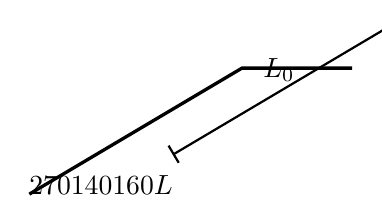
\begin{tikzpicture}
		
		\draw[very thick] (0,0)
		coordinate (a) 
		-- (2.7,1.6) 
		coordinate (b)
		-- (4.1,1.6)
		coordinate (c);
		
		
		\support{1}{a};
		\support{1}{c};
		
		\dimensioning{1}{a}{b}{-1}[$270\cml$];
		\dimensioning{1}{b}{c}{-1}[$140\cml$];
		\dimensioning{2}{a}{b}{2.7}[$160\cml$];
		\dimensioning{3}{a}{b}{1}[$L$];
		
		\draw[|-|, thick] (0,.5) -- (2.7,2.1)node[midway,above] {$L_{0}$} --
		(4.1,2.1);
		
		
		
		
	\end{tikzpicture}
	\caption{Schéma statique de l'escalier}
	\label{fig:schema-statique-escalier}
\end{figure}




\subsubsection{Dimensionnement des escaliers}



\textbf{Épaisseur des escaliers}

\[ \dfrac{L_{0}}{30} \leq e \leq \dfrac{L_{0}}{20} \]

Avec $L_{0}$ étant la portée de l'escalier.

\[ L = \sqrt{270^{2} + 160^{2}} = 313\cml \]

\[ L_{0} = L + 140 = 313 + 140 = 453\cml  \]

\vspace{\baselineskip}

\[ 15,1 \leq e \leq 22,65 \]

\[ \fbox{$e = 20\cml$} \]


\textbf{Dimensions des marches et contre-marche}

\[ 60 < g + 2 \times h < 64 \]

Avec g étant la longueur de la contre-marche et h la hauteur de la marche.

On pose : 

\[ \fbox{$h = 16\cml \quad;\quad g = 27\cml$} \]

\[ 58 < 27 + 2 \times 16 = 59\cml < 64 \]
{\centering Condition vérifiée.\par}

Nombre de marches = \underline{9 marches.}



\subsubsection{Calcul des charges}

\underline{Le calcul se fera pour 1ml.}

\vspace{\baselineskip}

\textbf{Charge permanente paillasse}

\begin{table}[H]
	\centering
	\caption{Les charges appliquées à la paillasse}
	\begin{tabular}{|l|c|c|}
		\hline
		\textbf{Nom de la charge} & \textbf{La charge} & \textbf{La charge appliqué}
		($\knm$) \\ \hline
		
		Poids propre & $25\knmc$ & $25 \times e \times 1ml = 25 \times 0,2 = 5$ \\
		\hline
		
		Poids des marches & $24\knmc$ & $24 \times h \times 1ml = 24 \times 0.16 =
		3,84 $ \\ \hline
		
		Couche de sable & $0,36\knms$ & 0,36 \\ \hline
		
		Mortier de pose & $0,44\knms$ & $2 \times 0,44$ \\ \hline
		
		Carrelage & $0,4\knms$ & $2 \times 0,4$ \\ \hline
		
		Garde corps & & 0,4 \\ \hline
		
		\multicolumn{2}{|l|}{\textbf{\textcolor{blue}{La somme}}} 
		& \textbf{\textcolor{blue}{11,28}} \\ \hline
		
		
	\end{tabular}
\end{table}



La charge du au mortier et au sable est multiplier par 2 car on aura ces deux
là sur la marche et aussi sur la contre-marche.





\vspace{\baselineskip}

\textbf{Charge permanente palier}


\begin{table}[H]
	\centering
	\caption{Les charges appliquées à la paillasse}
	\begin{tabular}{|l|c|c|}
		\hline
		\textbf{Nom de la charge} & \textbf{La charge} & \textbf{La charge appliqué}
		($\knm$) \\ \hline
		
		Poids propre & $25\knmc$ & $25 \times e \times 1ml = 25 \times 0,2 = 5$ \\
		\hline
		
		
		Couche de sable & $0,36\knms$ & 0,36 \\ \hline
		
		Mortier de pose & $0,44\knms$ & $0,44$ \\ \hline
		
		Carrelage & $0,4\knms$ & $0,4$ \\ \hline
		
		
		\multicolumn{2}{|l|}{\textbf{\textcolor{blue}{La somme}}} 
		& \textbf{\textcolor{blue}{2,64}} \\ \hline
		
		
	\end{tabular}
\end{table}



\vspace{\baselineskip}


\textbf{Charge d'exploitation}

Pour les escaliers on a :

\[ Q = 2,5\knms \rightarrow Q' = 2,5 \times 1ml = 2,5\knm \]


\vspace{\baselineskip}

\textbf{Charge totale à l'ELU}

Paillasse : $q_{paillasse} = 1,35 \times 11,28 + 1,5 \times 2,5 = 18,978 \simeq
19\knm $

\vspace{\baselineskip}

Palier : $q_{palier} = 1,35 \times 2,64 + 1,5 \times 2,5 = 7,314 \simeq
7,5\knm$


\[ \fbox{$\begin{aligned}
		q_{paillasse} &= 19\knm \\
		q_{palier} &= 7,5\knm
	\end{aligned}$} \]



\subsubsection{Calcul des efforts internes}



\begin{figure}[H]
	\centering
	\begin{tikzpicture}
		
		
		\draw[very thick] (0,0) 
		coordinate (a) --
		(4,0)
		coordinate (b) --
		(7,0)
		coordinate (c);
		
		\support{3}{a}[-90];
		\support{3}{c}[90];
		
		\lineload{1}{a}{b}[2][2];
		\lineload{1}{b}{c}[1][1];
		
		\dimensioning{1}{a}{b}{-1}[$3,13\meterl$];
		\dimensioning{1}{b}{c}{-1}[$1,4\meterl$];
		
		\node at (2,3) {$q = 19\knm$};
		\node at (5.8,1.8) {$q = 7,5\knm$};
		
	\end{tikzpicture}
\end{figure}

Pour facilité les calculs des effort internes on va considérer uniquement $q =
19\knm$ sur toute la travée.

\begin{figure}[H]
	\centering
	\begin{tikzpicture}
		
		
		\draw[very thick] (0,0) 
		coordinate (a) --
		(4,0)
		coordinate (b) --
		(7,0)
		coordinate (c);
		
		\support{3}{a}[-90];
		\support{3}{c}[90];
		
		\lineload{1}{a}{c}[2][2];
		
		\dimensioning{1}{a}{c}{-1}[$4,58\meterl$];
		
		\node at (3.5,3) {$q = 19\knm$};
		
		\node[left=.5] at (a) {A};
		\node[right=.5] at (c) {B};
		
		
	\end{tikzpicture}
\end{figure}



\textbf{Calcul des moments}

Sur les appuis :

\[ M_{A} = M_{B} = -\dfrac{q \times l^{2}}{12} = -\dfrac{19 \times
	4,53^{2}}{12} = -32,5\knxm \]

En travée :

\[ \mmt{A-B} = \dfrac{q \times l^{2}}{24} = \dfrac{19 \times 4,53^{2}}{24} =
16,24\knxm \]

\textbf{Efforts tranchants}

\[ V = \dfrac{q \times l}{2} = \dfrac{19 \times 4,53}{2} = 43\kn \]

\[ \fbox{$\begin{aligned}
		M_{A} = M_{B} &= -32 \knxm \\
		\mmt{A-B} &= 16 \knxm \\
		V &= 45 \kn
	\end{aligned}$} \]


\subsubsection{Calcul du ferraillage}

On a :
\begin{itemize}
	\item Hauteur de la section $h = 20\cml$
	\item Largeur de la section $b = 100\cml$
	\item Enrobage $c = 3\cml $
	\item $d = h - c = 20 - 3 = 17\cml$
\end{itemize}

\textbf{\underline{Armature longitudinale en travée}}

\[ \mu = \dfrac{\num{16e2}}{100 \times 17^{2} \times 1,42} = 0,039 < \mu_{l} =
0,392 \]
{\centering Section simplement armé\par}

\[ \alpha = 1,25 \times (1 - \sqrt{1 - 2 \times 0,039}) = 0,05 \rightarrow Z =
17 \times (1 - 0,4 \times 0,05) = 16,66\cml \]

\[ A_{st} = \dfrac{1600}{16,6 \times 34,8} = 2,77\cmsq \]




\textbf{Condition non fragilité}

\[ A_{\min} = 0,23 \times \dfrac{0,21}{40} \times 100 \times 17 = 2,05\cmsq \]

\[ \fbox{$A_{st} = 2,77\cmsq \rightarrow 6HA8 = 3,02\cmsq$} \]


{\centering Avec un espacement de $S_{l} = 15\cml$\par}

\vspace{\baselineskip}



\textbf{Vérification de l'adhérence des barres (A.6.1.3)}

\[ \tau_{se} = \dfrac{45}{0,9 \times 17 \times 6 \times \pi \times 0,8 } =
1,9\mpa < \taubar{se} = 3,15\mpa \]

{\centering Condition vérifié.\par}

\vspace{5\baselineskip}

\textbf{\underline{Armature longitudinale en appui}}

\[ \mu = \dfrac{\num{32e2}}{100 \times 17^{2} \times 1,42} = 0,078 < \mu_{l} =
0,392 \]
{\centering Section simplement armé\par}

\[ \alpha = 1,25 \times (1 - \sqrt{1 - 2 \times 0,078}) = 0,1\]

\[ \downarrow \]

\[ Z = 17 \times (1 - 0,4 \times 0,1) = 16,32\cml  \]

\[ A_{st} = \dfrac{1600}{16,32 \times 34,8} = 5,63\cmsq \]




\[ \fbox{$A_{st} = 5,63\cmsq \rightarrow 5HA12 = 5,65\cmsq$} \]


{\centering Avec un espacement de $S_{l} = 15\cml$\par}


\vspace{5\baselineskip}

\textbf{\underline{Armature de répartition}}

\[ A_{r} = \dfrac{A_{st}}{4} \]

En travée : $A_{r} = \dfrac{3,02}{4} = 0,755\cmsq \rightarrow 3HA6 = 0,85\cmsq$

En appui : $A_{r} = \dfrac{5,65}{4} = 1,41\cmsq \rightarrow 5HA6 = 1,41\cmsq$


\vspace{\baselineskip}

\textbf{\underline{Vérification au cisaillement}}

\[ \tau = \dfrac{V_{u}}{b \times d} = \dfrac{45}{100 \times 17} = 0,26\mpa < \taubar{u} = 3,33\mpa \]
{\centering Condition vérifié.\par}





\subsection{Poutres palières}

\subsubsection{Introduction}

Poutre d'un palier sur laquelle s'appuient les limons d'un escalier.

\vspace{\baselineskip}

Les dimensions de la poutre palière sont : $h = 35\cml$, $b = 20\cml$, $L = 3,4\meterl$, $c = 3\cml \rightarrow d = 32\cml$

\subsubsection{Calcul des charges}

La poutre reprend son poids propre + le mur en dessus et aussi la charge de l'escalier qui est la réaction déja calculer ($R = 45\kn$).

\vspace{\baselineskip}

La charge R est une charge concentrée, mais en réalité notre escalier se repose tout entier sur la poutre donc on doit divisé cette réaction tout au long de la poutre palière.

\begin{figure}[H]
	\centering
	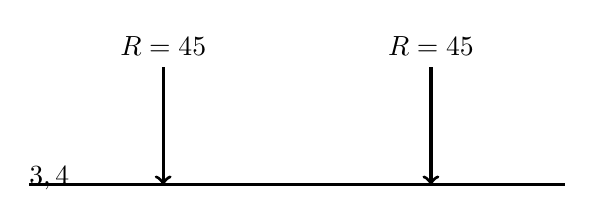
\begin{tikzpicture}
		
		
		\draw[very thick] (0,0) 
		coordinate (a) --
		(3.4,0)
		coordinate (b) --
		(6.8,0)
		coordinate (c);
		
		\support{3}{a}[-90];
		\support{3}{c}[90];
		
		
		\draw[very thick, <-] (1.7,0) coordinate (r1) -- (1.7,1.5) node[above] {$R = 45\kn$};
		\draw[very thick, <-] (5.1,0) coordinate (r2) -- (5.1,1.5) node[above] {$R = 45\kn$};
		
		\dimensioning{1}{a}{c}{-1}[$3,4\meterl$];
		
		
		
	\end{tikzpicture}
\end{figure}

On transforme les charges R en charges uniformément repartie : $q_{R} = \dfrac{45}{1,7} = 26,47\knm \simeq 26\knm$

\begin{figure}[H]
	\centering
	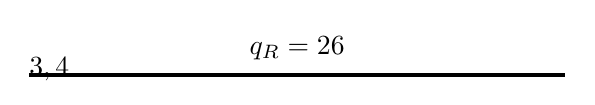
\begin{tikzpicture}
		
		
		\draw[very thick] (0,0) 
		coordinate (a) --
		(3.4,0) node[above=1.5] {$q_{R} = 26\knm$}
		coordinate (b) --
		(6.8,0)
		coordinate (c);
		
		\support{3}{a}[-90];
		\support{3}{c}[90];
		
		
		\lineload{1}{a}{c}[1][1];
		
		
		\dimensioning{1}{a}{c}{-1}[$3,4\meterl$];
		
		
		
	\end{tikzpicture}
\end{figure}

\vspace{2\baselineskip}


\textbf{Calcul du poids propre + mur}

\vspace{\baselineskip}

Poids propre :

\[ q_{pp} = 25 \times 0,35 \times 0,2 = 1,75\knm \]

Poids du mur :

\[ q_{mur} = 0,9\knms \times 0,2 = 0,18\knm \]

\vspace{2\baselineskip}

\textbf{Charge totale}

\[ q = 26 + 1,35 \times (1,75 + 0,18) = 28,6\knm \simeq 28\knm \]


\subsubsection{Schéma statique}

\begin{figure}[H]
	\centering
	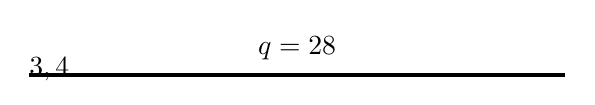
\begin{tikzpicture}
		
		
		\draw[very thick] (0,0) 
		coordinate (a) --
		(3.4,0) node[above=1.5] {$q = 28\knm$}
		coordinate (b) --
		(6.8,0)
		coordinate (c);
		
		\support{3}{a}[-90];
		\support{3}{c}[90];
		
		
		\lineload{1}{a}{c}[1][1];
		
		
		\dimensioning{1}{a}{c}{-1}[$3,4\meterl$];
		
		
		
	\end{tikzpicture}
\end{figure}


\subsubsection{Calcul des efforts internes}

\[ \fbox{$\begin{aligned}
		M_{A} = M_{B} &= -26,97\knxm \simeq -27\knxm \\
		\mmt{A-B} &= 13,48 \simeq 13,5\knxm \\
		V &= 47,6\kn
	\end{aligned}$} \]

\subsubsection{Calcul du ferraillage}

\textbf{\underline{Armature longitudinal en travée}}

\[ \mu = \dfrac{1350}{20 \times 32^{2} \times 1,42} = 0,046 < \mu_{l} = 0,392 \]
{\centering Section simplement armé\par}

\[ \begin{aligned}
	\alpha &= 1,25 \times (1 - \sqrt{1 - 2 \times 0,046}) = 0,059 \\
	Z &= 32 \times (1 - 0,4 \times 0,059) = 31,24\cml
\end{aligned} \]

\[ A_{st} = \dfrac{1350}{31,24 \times 34,8} = 1,24\cmsq \]

\textbf{Condition non fragilité}

\[ A_{\min} = \dfrac{0,21}{40} \times 20 \times 32 = 3,36\cmsq > A_{st} \]
{\centering Condition non vérifié\par}

\vspace{\baselineskip}

Donc finalement : \fbox{$A_{st} = A_{\min} = 3,36\cmsq \underset{\text{on choisie}}{\rightarrow} 3HA12 = 3,39\cmsq$}

\vspace{5\baselineskip}

\textbf{\underline{Armature en appui}}

\[ \mu = \dfrac{2700}{20 \times 32^{2} \times 1,42} = 0,093 < \mu_{l} = 0,392 \]
{\centering Section simplement armé\par}

\[ \begin{aligned}
	\alpha &= 1,25 \times (1 - \sqrt{1 - 2 \times 0,093}) = 0,122 \\
	Z &= 32 \times (1 - 0,4 \times 0,122) = 30,43\cml
\end{aligned} \]

\[ A_{st} = \dfrac{2700}{30,43 \times 34,8} = 2,55\cmsq \]

\textbf{Condition non fragilité}

\[ A_{\min} = \dfrac{0,21}{40} \times 20 \times 32 = 3,36\cmsq > A_{st} \]
{\centering Condition non vérifié\par}

\vspace{\baselineskip}

Donc finalement : \fbox{$A_{st} = A_{\min} = 3,36\cmsq \underset{\text{on choisie}}{\rightarrow} 3HA12 = 3,39\cmsq$}

\vspace{3\baselineskip}

\textbf{\underline{Vérification au cisaillement}}

\[ \tau = \dfrac{V_{u}}{b \times d} = \dfrac{47600}{200 \times 320} = 0,74\mpa < \taubar{u} = 3,33\mpa \]
{\centering Condition vérifié.\par}


\vspace{6\baselineskip}


\textbf{\underline{Armature transversale}}

\[ \varPhi_{t} = \min \begin{cases}
	\dfrac{h}{35} = 1\cml\\
	\varPhi_{l} = 1,2\cml \\
	\dfrac{b}{10} = 2\cml
\end{cases} \]

\[ \varPhi_{t} = 1\cml = 10\mm \]

On choisie pour les armatures transversales : $1HA10 = 0,79\cmsq$

Avec un espacement de :

\[ S_{t} = \begin{cases}
	15\varPhi_{l} = 15 \times 1,2 = 18\cml \\
	40\cml \\
	\text{Plus petite dimension  + 10cm} = 20 + 10 = 30\cml
\end{cases} \]

\[ S_{t} = 18\cml \rightarrow 20\cml \]

\vspace{2\baselineskip}

\textbf{Le \cite[7.5.2.2]{rpa} préconise pour les poutre :}

\[ A_{t} = 0,003 \times S_{t} \times b \]

Avec : Dans les zones nodales : $S_{t} = \min \begin{cases}
	\dfrac{h}{4} = \dfrac{35}{4} = 8,75\cml \\
	12 \times \varPhi_{l} = 14,4\cml
\end{cases} = 10\cml$

En dehors des zones nodales : $S_{t} \leq \dfrac{35}{2} = 17,5\cml = 15\cml$

\[ A_{t} = 0,003 \times 15 \times 20 = 0,9\cmsq \]

\[ \fbox{$A_{t}^{RPA} > A_{t}^{BAEL}$} \]
{\centering Finalement on choisie $A_{t} = 0,9\cmsq$\par}

\vspace{\baselineskip}

Avec $A_{t} = 0,9\cmsq \underset{\text{on choisie}}{\rightarrow} 4HA6 = 1,13\cmsq$ (Cadre + étrier)

\vspace{\baselineskip}

Avec un espacement de 10 au zone nodale (les première armature seront disposé à 5cm du nu d'appui), et en zone courante à 15cm.




\subsection{Plan de ferraillage}

Pour résumé :

\begin{table}[H]
	\caption{Résumé du ferraillage des escaliers et des poutres palières}
	\label{tab:resume-ferraillage-escalier-poutre}
	\begin{tabular}{|l|c|c|c|c|c|}
		\hline
		Éléments & \multicolumn{2}{|c|}{Armatures longitudinales} & \multicolumn{3}{|c|}{Armatures transversales} \\ \hline
	 
	 & Travée & Appui & Travée & Appuie & Espacement \\ \hline
	 
		Escalier & 6HA8 ($S_{t} = 15\cml$) & 5HA12 ($S_{t} = 15\cml$) & 3HA6 & 5HA6 & \\ \hline
		
		Poutre P & 3HA12 & 3HA12 & 4HA6 & 4HA6 & 5cm--10cm--15cm \\ \hline
	\end{tabular}
\end{table}


\begin{figure}
	\centering
	\includegraphics[width=1\linewidth]{"figures/Chapitre 3/ferraillage-escalier"}
	\caption{Plan de ferraillage des escaliers et de la poutre palière}
	\label{fig:ferraillage-escalier}
\end{figure}



